\documentclass[german]{latteachCD}
\usepackage{mdframed}
\usepackage{amsmath}
\usepackage{amsfonts}
\usepackage{amssymb}
\usepackage{fdsymbol}
%\usepackage{wasysym}
%\usepackage{stmaryrd}
%\usepackage{fixltx2e}
%\usepackage{enumitem}
%\usepackage{extarrows}
%\newcommand{\abs}[1]{\lvert#1\rvert}

\usepackage{tikz}
\usetikzlibrary{arrows,automata,positioning,shapes,calc,decorations.pathmorphing,matrix}

\tikzstyle{automaton}=[->, >=stealth', initial text=, auto, node distance=20mm, bend angle=20, semithick, x=20mm, y=20mm]
\tikzset{
  every state/.style={
    inner sep=0pt,
    minimum size=8mm
  },
  small state/.style={
      state,
      minimum size=3mm
  },
  ellipse state/.style={
    draw,
    shape=ellipse,
    minimum width=20mm,
    minimum height=12.36mm,
    text width=14.5mm,
    inner sep=0mm,
    path picture={
      \draw (path picture bounding box.east) ellipse [x radius=9mm, y radius=9mm];
    }
  },
  accepting ellipse state/.style={
    ellipse state,
    path picture={
      \clip (path picture bounding box.east) ellipse [x radius=9.4mm, y radius=9.4mm];
      \draw[double] (path picture bounding box.east) ellipse [x radius=9mm, y radius=9mm];
      \draw[double] (path picture bounding box.center) ellipse [x radius=10mm, y radius=6.18mm];
    }
  }
}


%%%%%%%%%%%%%%%%%%%%%%%%%%%%%%%%%%%%%%%%%%%%%%%%%%%%%%%%%%%%%%%%%%%%%%%%%%%%%%%%%%%%%%%%%%%%

\usepackage{xspace}

\author{~}
\term{Wintersemester 2017/18}
\title{\Large 6.\@ Übungsblatt}
\course{\LARGE Formale Systeme}

\usepackage{csquotes}
\usepackage{booktabs}
\usepackage{amsmath}
\usepackage{amsfonts}
\usepackage{amssymb}
\usepackage{mathtools}
\usepackage{wasysym}
\usepackage{stmaryrd}
\usepackage{enumitem}
\usepackage{tikz}
\usepackage{makecmds}

\renewcommand{\epsilon}{\varepsilon}
\renewcommand{\phi}{\varphi}
\renewcommand{\rho}{\varrho}
\renewcommand{\theta}{\vartheta}
\newcommand{\tuple}[1]{\langle{#1}\rangle} 

\newcommand{\size}[1]{\ensuremath{\lvert #1\rvert}}
\newcommand{\gdw}{\mathrel{\mathrm{gdw.}}}
\newcommand{\falls}{\mathrel{\mathrm{falls}}}

\provideenvironment{solution}{\textbf{Lösung}:}{}
\usepackage{comment}

\usepackage{etex,etoolbox}

\DeclareRobustCommand{\NN}{\ensuremath{\mathbb{N}}}

\newbool{Baader}
\newbool{Kroetzsch}
\booltrue{Kroetzsch}

\DeclareMathOperator{\Var}{Var}
\ifbool{Baader}{%
  \DeclareMathOperator{\Unt}{Unt}
  \DeclareMathOperator{\Res}{Res}
}{}
\ifbool{Kroetzsch}{%
  \DeclareMathOperator{\Unt}{Sub}
  \DeclareMathOperator{\Res}{Res}
  \usepackage{multicol}         % for resolution
}{}

\excludecomment{solution}

\begin{document}

\maketitle

\begin{center}
\begin{mdframed}
  \renewcommand{\theexercise}{zur Selbstkontrolle
  (diese werden in den Übungen nicht besprochen)}
  
\begin{exercise}
\begin{enumerate}
\item[S11)] Sei $\Sigma_1 = \{a,b\}$ und $\Sigma_2 =\{a,b,c\}$. Geben Sie für jede der folgenden Sprachen
  $L_i$ einen regulären Ausdruck $\alpha_i$ mit $L_i=L(\alpha_i)$ an. Begr\"unden
  Sie die von Ihnen gew\"ahlten regulären Ausdrücke $\alpha_i$.
                                %
  \begin{enumerate}
  \item $L_1 = \{ w\in \Sigma_1^* \mid w \text{ beginnt mit}\; a \text{ und }
    |w|_b \text{ ist gerade}\}$
  \item $L_2 = \{ w\in \Sigma_2^* \mid w \text{ beginnt mit}\; a \text{ und }
    |w|_b \text{ ist gerade}\}$
  \item $L_3 = \{ w\in \Sigma_1^* \mid \text{es gibt kein} \;u,v\in
    \Sigma_1^* \text{ mit} \;w=uaav\}$
  \item $L_4 = \{ w\in \Sigma_2^* \mid \text{es gibt kein} \;u,v\in \Sigma_2^* \text{ mit} \;w=uaav\}$

\end{enumerate}
\item[S12)] Wiederholen Sie die Begriffe Potenzmengenkonstruktion, erreichbarer Zustand, äquivalente Zustände, Quotientenautomat, reduzierter Automat und
  {\emph{Nerode}}-Rechtskongruenz.
\end{enumerate}

\end{exercise}

%  {\bfseries Hinweis:} Die Aufgaben *) und **)
%  dienen der Selbstkontrolle und werden in der
%  Übung nicht besprochen.
\end{mdframed}
\end{center}

\setcounter{exercise}{0}

\newpage

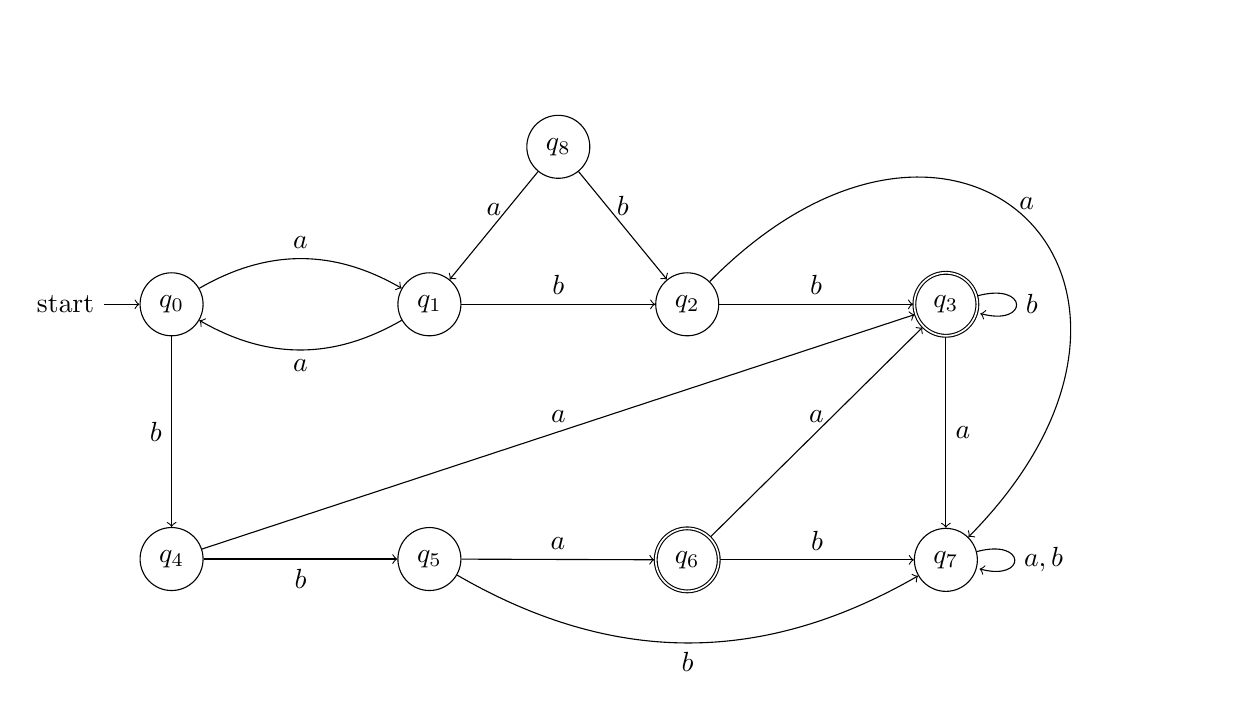
\begin{tikzpicture}[node distance=16ex and 7em]
    \path{
      node[state,initial] (q_0) {$q_0$}
      node[state] (q_1) [right=of q_0]{$q_1$}
      node[state] (q_2) [right=of q_1]{$q_2$}
      node[state] (q_8) at ($(q_1)!0.5!(q_2)+(0,2)$) {$q_8$}
      node[state,accepting] (q_3) [right=of q_2]{$q_3$}
      node[state] (q_4) [below=of q_0]{$q_4$}
      node[state] (q_5) [below=of q_1]{$q_5$}
      node[state,accepting] (q_6) [below=of q_2]{$q_6$}
      node[state] (q_7) [below=of q_3]{$q_7$}
    };

    \path[->,draw]{
      (q_0) edge node[left]{$b$}  (q_4)
      (q_1) edge node[above]{$b$} (q_2)
      (q_2) edge node[above]{$b$} (q_3)
      (q_3) edge node[right]{$a$} (q_7)
      (q_4) edge node[below]{$b$} (q_5)
      (q_5) edge node[above]{$a$} (q_6)
      (q_6) edge node[above]{$b$} (q_7)
      (q_4) edge node[above]{$a$} (q_3)
      (q_6) edge node[above]{$a$} (q_3)
      (q_0) edge[bend left] node[above]{$a$} (q_1)
      (q_1) edge[bend left] node[below]{$a$} (q_0)
      (q_2) edge[bend left=90,looseness=2.5] node[above]{$a$} (q_7)
      (q_7) edge[loop right] node {$a,b$} (q_7)
      (q_5) edge[bend right=30] node[below]{$b$} (q_7)
      (q_8) edge node[above]{$b$}(q_2)
      (q_8) edge node[above]{$a$}(q_1)
      (q_3) edge[loop right] node {$b$} (q_3)
    };
  \end{tikzpicture}


\begin{exercise}
Beweisen oder widerlegen Sie unter Verwendung von Resultaten aus der Vorlesung folgende Aussagen.
\begin{enumerate}
\item F\"ur die Grammatik $G=(\{S,X,Y,Z\},\{a,b\},\{S\rightarrow Y,\;X\rightarrow b,\;Y\rightarrow aYYb,\;aY\rightarrow aZ,\;ZY\rightarrow ZX,\;Z\rightarrow a\},S)$ gilt: $abab\in L(G)$.
\item Kann eine Sprache $L$ von einem DFA erkannt werden, so gibt es auch einen
  $\varepsilon$-NFA $\mathcal M$ mit $L({\mathcal M})=L$.
\item F\"ur jeden NFA $\mathcal M$ mit Wort\"uberg\"angen gibt es einen \"aquivalenten NFA.
\item Es gibt eine regul\"are Sprache, f\"ur welche die Anzahl der \"Aquivalenzklassen der zugeh\"origen {\emph{Nerode}}-Rechtskongruenz endlich ist.
\item Wenn es f\"ur eine Sprache $L$ ein $n\in \mathbb N$ gibt, so dass die {\emph{Nerode}}-Rechtskongruenz $\simeq_L$ höchstens $n$ Äquivalenzklassen hat, so
  kann $L$ von einem DFA erkannt werden.
\item F\"ur jede Sprache $L$ gilt: $L = \bigcup\limits_{u \in L} [u]_{\simeq_{L}}\;$, d.\,h. $L$ ist die Vereinigung von $\simeq_{L}$-Klassen.
\end{enumerate}
\end{exercise}



% kam wohl schon in der vorlesung vor - rausgenommen:
%\input{pool/sprachen-dfa-eigenschaften}

\newpage

\begin{exercise}
Gegeben ist das Alphabet $\Sigma = \{a,b\}$. Welche der folgenden
Sprachen $L_i$ \"uber $\Sigma$ mit $1\le i\le 3$ ist regul\"ar? Beweisen Sie Ihre jeweilige
Antwort.
\begin{itemize}
\item[a)] $L_1=\{a^ib^i\mid i\ge 1\}$
\item[b)] $L_2=\{xyz\mid  x,y\in \Sigma^*, \ |x|\ge 1,|y|\ge 1, z=sp(x)\}\;\;\;$\\
{\emph{Hinweis}}: $sp(x)$ bildet das Spiegelwort zu $x$.
\item[c)] $L_3=\{a^{i^2}\mid i\ge 1\}$
\end{itemize}
\end{exercise}



\begin{exercise}
Gegeben ist der NFA $\mathcal M=(\{q_0,q_1,q_2,q_3,q_4\},\{a,b,c,d\}, \delta ,\{q_0\},\{q_2\})$ mit $\delta$:
\vspace*{0.5cm}
\begin{center}
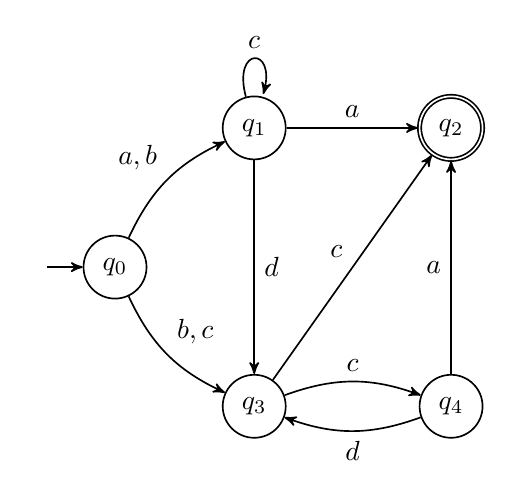
\begin{tikzpicture} [->, >=stealth', initial text=, auto, node
  distance=25mm, bend angle=20, semithick]%[node distance=2cm,auto]
 
 \node[state,initial] (q_0) {$q_0$}; 
 \node[state] (q_1) [above right of=q_0] {$q_1$}; 
 \node[state,accepting] (q_2) [right of=q_1] {$q_2$}; 
 \node[state] (q_3) [below right of=q_0] {$q_3$};
 \node[state] (q_4) [right of=q_3] {$q_4$};
      
  \path[->]
  (q_0) edge [bend left]  node {$a, b$} (q_1) 
  (q_0) edge  [bend right] node {$b, c$} (q_3) 
  (q_1) edge [loop above] node {$c$} (q_1) 
  (q_1) edge node {$a$} (q_2) 
  (q_1) edge node {$d$} (q_3) 
  (q_3) edge node {$c$} (q_2) 
  (q_3) edge [bend left] node {$c$} (q_4) 
  (q_4) edge  node {$a$} (q_2)
  (q_4) edge [bend left] node {$d$} (q_3);
\end{tikzpicture}
\end{center}
Geben Sie für jedes $z\in \{bc,adc,cda,bcdc,acdc\}$ alle Zerlegungen $z=uvw$ mit
$u,w\in \Sigma^*$, $v\in \Sigma^{+}$ an, sodass für alle $k\ge 0$ gilt:
$uv^kw\in L(\mathcal M)$. Begründen Sie Ihre Antworten.
\end{exercise}


\end{document}
